\subsection{Additive approach}

\begin{frame}{Additive approach}
	\textbf{Variational Problem :} Let $u_{\theta} \in H^{k+1}(\Omega)\cap H^1_0(\Omega)$.
	
	\vspace{-5pt}
	\begin{equation}
		\label{eq:weakplus}
		\text{Find } p_h^+ \in V_h^0 \text{ such that}, \forall v_h \in V_h^0, a(p_h^+,v_h) = l(v_h) - a(u_{\theta},v_h),\tag{$\mathcal{P}_h^+$}
	\end{equation}
	
	\vspace{5pt}
	\begin{minipage}[t]{0.6\linewidth}
		with the \textcolor{red}{enriched trial space $V_h^+$} defined by
		\begin{equation*}
			V_h^+ = \left\{
			u_h^+= u_{\theta} + p_h^+, \quad p_h^+ \in V_h^0
			\right\}.
		\end{equation*}
	
		\vspace{20pt}
	
		\textbf{General Dirichlet BC :} If $u=g$ on $\partial \Omega$, then
		\[
			p_h^+ = g - u_{\theta} \text{\quad on } \partial \Omega,
		\]
		with $u_\theta$ the PINN prior. 
	\end{minipage} \qquad \begin{minipage}[t][][b]{0.28\linewidth}
		\vspace{-15pt}
		\centering
		\pgfimage[width=\linewidth]{images/correction/correction.pdf}
	\end{minipage}
\end{frame}

\begin{frame}{Convergence analysis}
	\vspace{-10pt}
	\hypersetup{
		citecolor=white,
	}

	\begin{mytheo}{Convergence analysis of the standard FEM \footnotesize\citep{Ern2004TheoryAP}\normalsize}{fem}
		We denote $u_h\in V_h$ the solution of \eqref{eq:weakform} with $V_h$ the standard trial space. Then,
		\vspace{-5pt}
		\begin{equation*}
			| u-u_h|_{H^1} \leqslant C_{H^1} \, h^{k} |u|_{H^{k+1}},
		\end{equation*}
		\begin{equation*}
			\| u-u_h\|_{L^2} \leqslant C_{L^2} \, h^{k+1} |u|_{H^{k+1}}.
		\end{equation*}
	\end{mytheo}
	
	\begin{mytheo}{Convergence analysis of the enriched FEM \footnotesize\citep{ours_2025}\normalsize}{add}
		We denote $u_h^+\in V_h^+$ the solution of \eqref{eq:weakplus} with $V_h^+$ the enriched trial space. Then,
		\vspace{-5pt}
		\begin{equation*}
			| u-u_h^+|_{H^1} \leqslant \fcolorbox{orange}{other!10!white}{$\frac{| u-u_{\theta} |_{H^{k+1}}}{| u |_{H^{k+1}}}$} \left(C_{H^1} \, h^{k} |u|_{H^{k+1}}\right),
		\end{equation*}
		\begin{equation*}
			\| u-u_h^+\|_{L^2} \leqslant \fcolorbox{orange}{other!10!white}{$\frac{| u-u_{\theta} |_{H^{k+1}}}{| u |_{H^{k+1}}}$} \left(C_{L^2} \, h^{k+1} |u|_{H^{k+1}}\right).
		\end{equation*}
	\end{mytheo}

	\hypersetup{
		citecolor=other,
	}

	\footnotesize
	\textcolor{orange}{Gains of the additive approach.}
\end{frame}

\subsection{\filledstar Numerical results}

\begin{frame}{1st problem considered} 
	\textbf{Problem statement:} Considering an \textcolor{red}{Anisotropic Elliptic problem with Dirichlet BC}:
	\vspace{-5pt}
	\begin{equation*}
		\left\{
		\begin{aligned}
			-\text{div}(D\nabla u) & = f, \; &  & \text{in } \; \Omega, \\
			u         & =0, \;  &  & \text{on } \; \partial\Omega,
		\end{aligned}
		\right.
		% \label{eq:Ell2D}\tag{$\mathcal{P}$}
	\end{equation*}

	with $\Omega=[0,1]^2$ and $\mathcal{M}=[0.4, 0.6]\times [0.4, 0.6]\times [0.01,1]\times [0.1,0.8]$ ($p=4$).
	
	\vspace{8pt}
	\textbf{Right-hand side :}

	\vspace{-5pt}
	\begin{equation*}
		f(\bm{x},\bm{\mu})=\exp\left(-\frac{(x-\mu_1)^2+(y-\mu_2)^2}{0.025\sigma^2}\right).
	\end{equation*}
	
	\textbf{Diffusion matrix :} (symmetric and positive definite)
	\begin{equation*}
		D(\bm{x},\bm{\mu})=\begin{pmatrix}
			\epsilon x^2+y^2 & (\epsilon-1)xy \\
			(\epsilon-1)xy & x^2+\epsilon y^2
		\end{pmatrix}.
	\end{equation*}

	\vspace{2pt}
	\small
	\textbf{PINN training:} Imposing BC exactly with a level-set function.
\end{frame}

\begin{frame}{Numerical results}
	\hspace{-5pt}\begin{minipage}[t]{0.46\linewidth}
		\textbf{Error estimates :} 1 set of parameters.
		$$\bm{\mu}=(0.51,0.54,0.52,0.55)$$
		\vspace{-35pt}
		\begin{figure}[H]
			\cvgFEMCorrAlldeg{images/numeric/elliptic/cvg/FEM_case3_v1_param1.csv}{images/numeric/elliptic/cvg/Corr_case3_v1_param1.csv}{1e-9}
		\end{figure}
	\end{minipage} \qquad \small
	\begin{minipage}[t]{0.48\linewidth}
	\end{minipage}
\end{frame}

\begin{frame}[noframenumbering]{Numerical results}
	\hspace{-5pt}\begin{minipage}[t]{0.46\linewidth}
		\textbf{Error estimates :} 1 set of parameters.
		$$\bm{\mu}=(0.51,0.54,0.52,0.55)$$
		\vspace{-35pt}
		\begin{figure}[H]
			\cvgFEMCorrAlldeg{images/numeric/elliptic/cvg/FEM_case3_v1_param1.csv}{images/numeric/elliptic/cvg/Corr_case3_v1_param1.csv}{1e-9}
		\end{figure}
	\end{minipage} \qquad \small
	\begin{minipage}[t]{0.48\linewidth}
		\textbf{Gains achieved :} $n_p=50$ sets of parameters.
		$$\mathcal{S}=\left\{\bm{\mu}^{(1)},\dots,\bm{\mu}^{(n_p)}\right\}$$
		\vspace{-15pt}
		\begin{table}[H]
			\gainstableallq{images/numeric/elliptic/gains/Tab_stats_case3_v1.csv}
		\end{table}

		\normalsize\centering\vspace{-20pt}
		$$N=20$$

		\vspace{-5pt}
		Gain : $\| u-u_h\|_{L^2} / \| u-u_h^+\|_{L^2}$ \\
		
		\small\vspace{8pt}
		Cartesian mesh : $N^2$ nodes.
	\end{minipage}
\end{frame}

\begin{frame}{2nd problem considered} 
	\textbf{Problem statement:} Considering the \textcolor{red}{Poisson problem with mixed BC}:
	\vspace{-5pt}
	\begin{equation*}
		\left\{
		\begin{aligned}
			-\Delta u & = f, \; &  & \text{in } \; \Omega \times \mathcal{M}, \\
			u         & = g, \;  &  & \text{on } \; \Gamma_E \times \mathcal{M}, \\
			\smash{\frac{\partial u}{\partial n}}+u  & = g_R, \;  &  & \text{on } \; \Gamma_I \times \mathcal{M},
		\end{aligned}
		\right.
		% \label{eq:Lap2DMixed}\tag{$\mathcal{P}$}
	\end{equation*}

	with $\Omega=\{(x,y)\in\mathbb{R}^2, \; 0.25\le x^2+y^2\le 1\}$ and $\mathcal{M}=[2.4,2.6]$ ($p=1$).
		
	\vspace{8pt}
	\textbf{Analytical solution :}

	\vspace{-12pt}
	\begin{equation*}
		% \label{eq:analytical_solution_Lap2D}
		u(\bm{x};\bm{\mu})= 1 - \frac{\ln\big(\mu_1\sqrt{x^2+y^2}\big)}{\ln(4)},
	\end{equation*}
	\vspace{-5pt}
	
	\textbf{Boundary conditions :}
	\begin{equation*}
		g(\bm{x};\bm{\mu})=1 - \frac{\ln(\mu_1)}{\ln(4)} \quad \text{and} \quad g_R(\bm{x};\bm{\mu})=2 + \frac{4-\ln(\mu_1)}{\ln(4)}.
	\end{equation*}

	\vspace{2pt}
	\small
	\textbf{PINN training:} Imposing mixed BC exactly in the PINN\footcite{Sukumar_2022}.

	\vspace{8pt}
\end{frame}

\begin{frame}{Numerical results}
	\hspace{-5pt}\begin{minipage}[t]{0.46\linewidth}
		\textbf{Error estimates :} 1 set of parameters.
		$$\bm{\mu}=2.51$$
		\vspace{-35pt}
		\begin{figure}[H]
			\cvgFEMCorrAlldeg{images/numeric/poisson/mixed/cvg/FEM_case5_v2_param1.csv}{images/numeric/poisson/mixed/cvg/Corr_case5_v2_param1.csv}{1e-10}
		\end{figure}
	\end{minipage} \qquad \small
	\begin{minipage}[t]{0.48\linewidth}
		\textbf{Gains achieved :} $n_p=50$ sets of parameters.
		$$\mathcal{S}=\left\{\bm{\mu}^{(1)},\dots,\bm{\mu}^{(n_p)}\right\}$$
		\vspace{-15pt}
		\begin{table}[H]
			\gainstableallq{images/numeric/poisson/mixed/gains/Tab_stats_case5_v2.csv}
		\end{table}

		\normalsize\centering\vspace{-20pt}
		$$h=1.33\cdot 10^{-1}$$

		\vspace{-5pt}
		Gain : $\| u-u_h\|_{L^2} / \| u-u_h^+\|_{L^2}$ \\
		\end{minipage}
\end{frame}

\begin{frame}{Numerical solutions}
	\vspace{-3pt}
	\textbf{1st problem :} $\bm{\mu}=(0.46,0.52,0.05,0.12)$

	\vspace{-8pt}
	\begin{figure}[!ht] \centering
		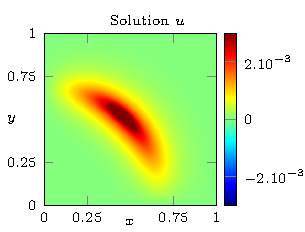
\includegraphics[width=0.34\linewidth]{images/numeric/elliptic/plots/solution.pdf}		
		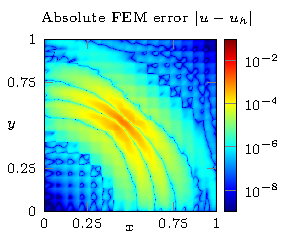
\includegraphics[width=0.31\linewidth]{images/numeric/elliptic/plots/error_FEM.pdf}	
		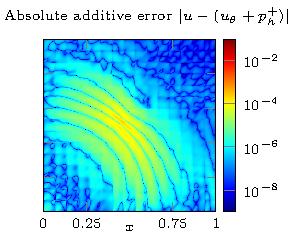
\includegraphics[width=0.31\linewidth]{images/numeric/elliptic/plots/error_ADD.pdf}	
	\end{figure}

	\vspace{-3pt}
	\textbf{2nd problem :} $\bm{\mu}=2.51 $

	\vspace{-8pt}
	\begin{figure}[!ht] \centering
		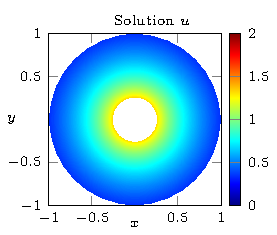
\includegraphics[width=0.31\linewidth]{images/numeric/poisson/mixed/plots/solution.pdf}		
		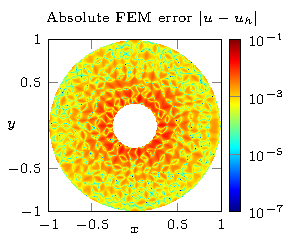
\includegraphics[width=0.31\linewidth]{images/numeric/poisson/mixed/plots/error_FEM.pdf}	
		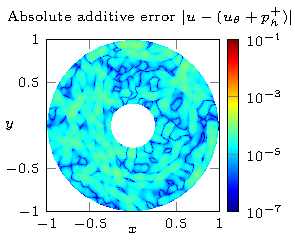
\includegraphics[width=0.31\linewidth]{images/numeric/poisson/mixed/plots/error_ADD.pdf}	
	\end{figure}

	% \begin{figure}[!ht] \centering
	% 	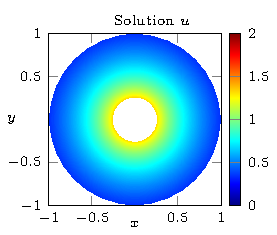
\includegraphics[width=0.31\linewidth]{images/numeric/poisson/mixed/plots/standalone_solutions_cropped.pdf}
	% 	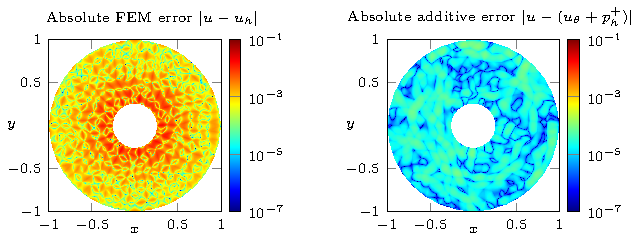
\includegraphics[width=0.7\linewidth]{images/numeric/poisson/mixed/plots/standalone_errors.pdf}
	% \end{figure}

	% \vspace{-8pt}
	% $$\bm{\mu}^{(1)}=2.51 $$
\end{frame}